\ifmostrarGabarito
\textbf{Resposta: (B)}

\textbf{Justificativa:}
Os índices da string \code{"PROGRAMACAO"} (tamanho 11) são:
\texttt{P(0), R(1), O(2), G(3), R(4), A(5), M(6), A(7), C(8), A(9), O(10)}.

A operação de fatiamento \code{s[1:8:2]} seleciona os elementos a partir do índice de início 1 até antes do índice de parada 8, com passo 2:
\begin{itemize}
    \item Índice 1: \code{'R'}
    \item Índice 3: \code{'G'}
    \item Índice 5: \code{'A'}
    \item Índice 7: \code{'A'}
\end{itemize}
Concatenando os caracteres selecionados, o resultado é \code{"RGAA"}.
\else
\par\vspace{0.15cm}
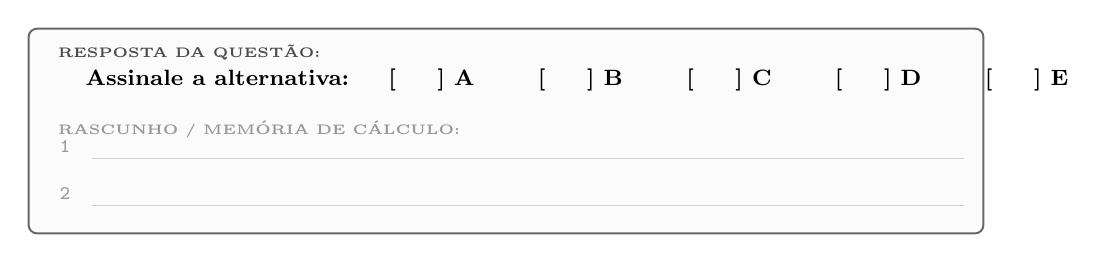
\begin{tikzpicture}
  \draw[rounded corners=3pt, draw=black!60, line width=0.7pt, fill=gray!3] (0,0) rectangle (\linewidth, -2.6cm);
  \node[anchor=north west, font=\tiny\bfseries\color{black!70}] at (0.25cm, -0.08cm) {RESPOSTA DA QUESTÃO:};
  \node[anchor=west, font=\footnotesize\bfseries] at (0.6cm, -0.65cm) {Assinale a alternativa: \quad [ \hspace{0.3cm} ] A \qquad [ \hspace{0.3cm} ] B \qquad [ \hspace{0.3cm} ] C \qquad [ \hspace{0.3cm} ] D \qquad [ \hspace{0.3cm} ] E};
  \node[anchor=north west, font=\tiny\bfseries\color{gray!80}] at (0.25cm, -1.05cm) {RASCUNHO / MEMÓRIA DE CÁLCULO:};
  \draw[gray!35, line width=0.4pt] (0.8cm, -1.65cm) -- (\linewidth-0.25cm, -1.65cm);
  \draw[gray!35, line width=0.4pt] (0.8cm, -2.25cm) -- (\linewidth-0.25cm, -2.25cm);
  \node[anchor=east, font=\scriptsize\ttfamily\color{gray!80}] at (0.65cm, -1.5cm) {1};
  \node[anchor=east, font=\scriptsize\ttfamily\color{gray!80}] at (0.65cm, -2.1cm) {2};
\end{tikzpicture}
\par\vspace{0.2cm}
\fi
